Una plataforma en la Nube para la administraci�n y localizaci�n de estacionamiento (SAE) capaz de ajustarse a las necesidades de las diferentes modalidades de estacionamientos  p�blicos y privados del Distrito  Federal como son estacionamiento, parqu�metros, valet-parking y  pensiones.  Permitir�  gestionar  y  realizar  las  tareas operativas y administrativas que se realizan de manera general en un estacionamiento. Figura \ref{fig:ArquitecturaGeneralSAE}

\begin{figure}[h]
	\centering
	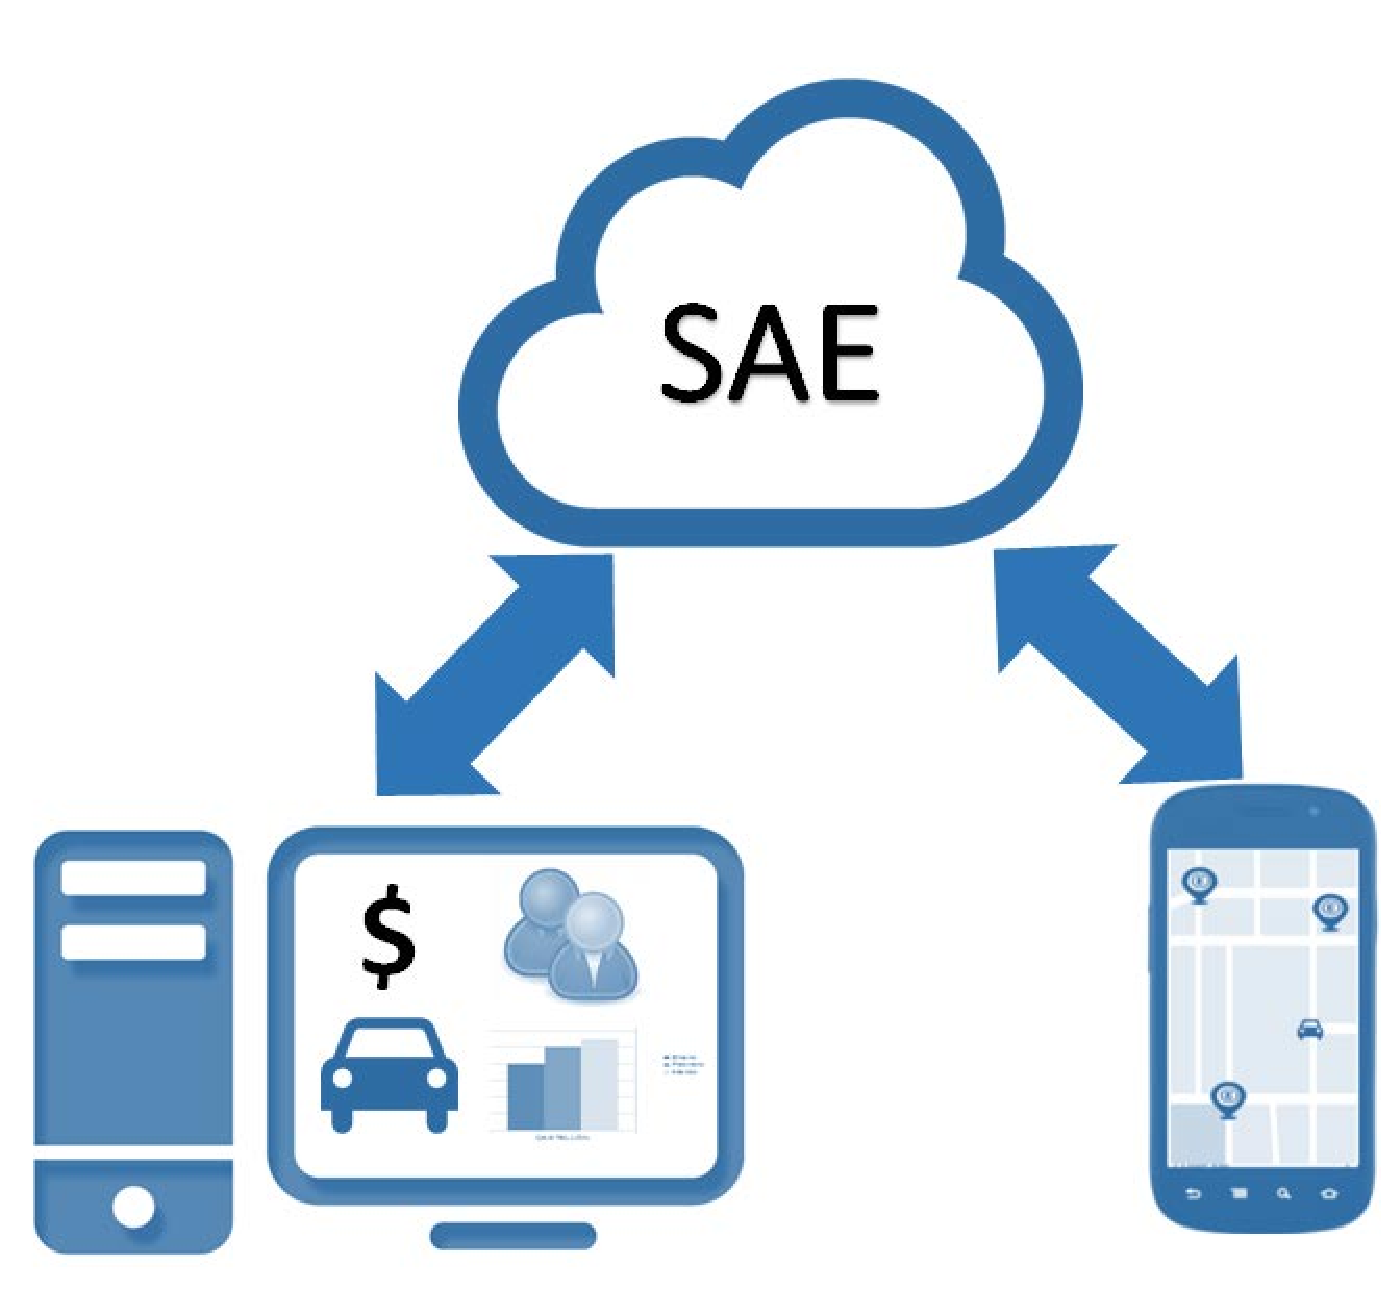
\includegraphics[scale=.4]{./definicionDelProducto/source/arquitecturaSAE.pdf}
	\caption{Arquitectura general SAE}
	\label{fig:ArquitecturaGeneralSAE}
\end{figure}		 

La informaci�n de los estacionamientos en operaci�n podr� ser visualizada por los usuarios finales a trav�s de una app m�vil de manera f�cil. Esta mostrar� en un mapa los estacionamientos cercamos, n�mero de cajones disponibles, horarios, modos de cobro, tarifas, y una calificaci�n.Figura \ref{fig:usuarioAppLocalizacion}

\begin{figure}[ht]
	\centering
	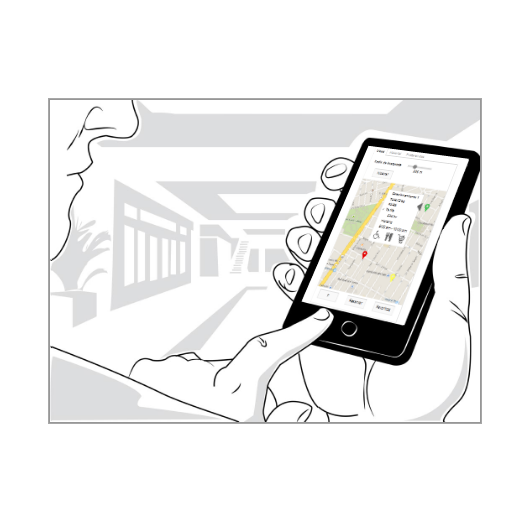
\includegraphics[scale=0.4]{./definicionDelProducto/source/usuarioApp}
	\caption{App de localizaci�n}
	\label{fig:usuarioAppLocalizacion}
\end{figure}

\newpage
La Figura \ref{fig:EscenarioSAE} ejemplifica el escenario principal de uso del SAE.

\begin{figure}[ht]
	\centering
	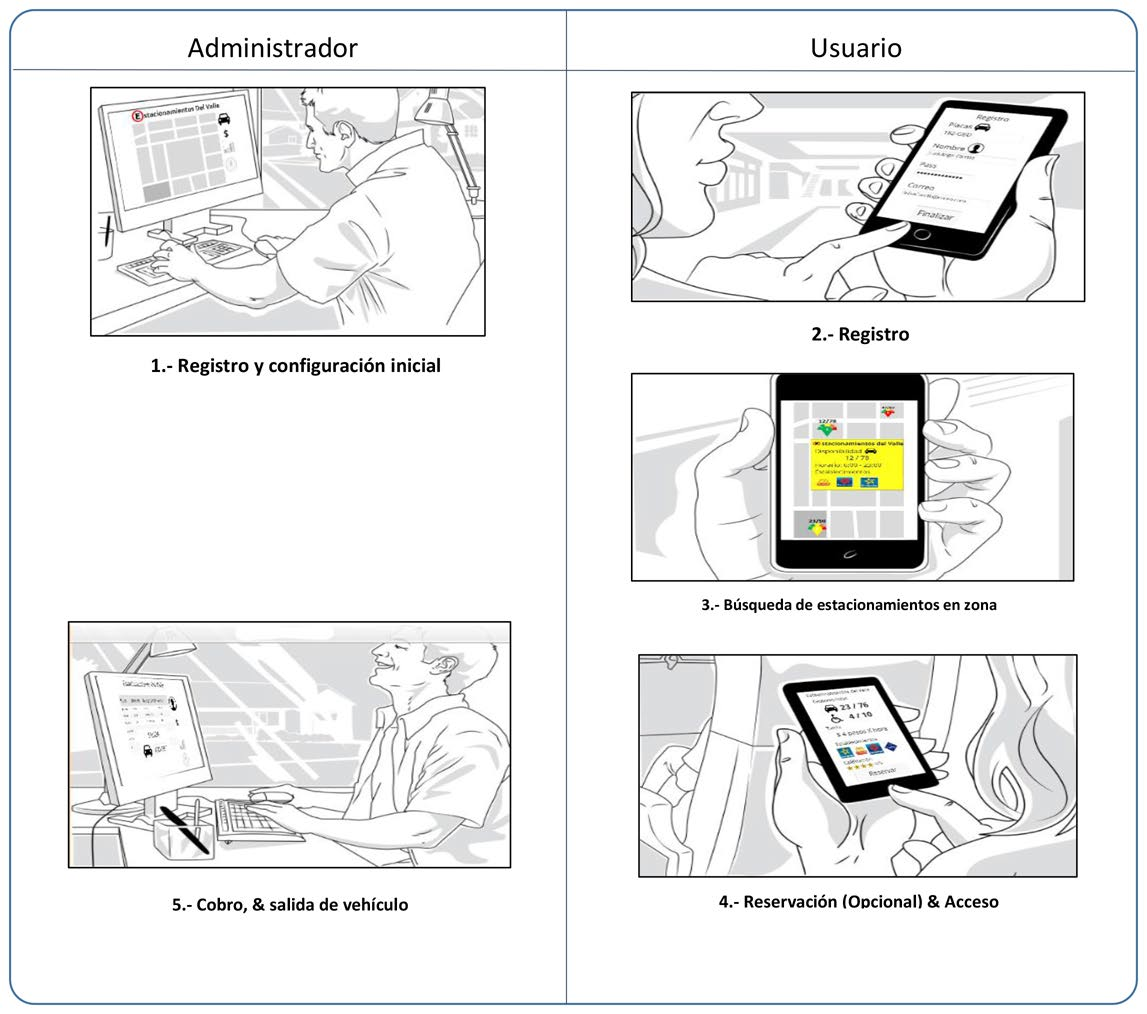
\includegraphics[scale=0.75]{./definicionDelProducto/source/storyboard.pdf}
	\caption{Escenario de uso SAE}
	\label{fig:EscenarioSAE}
\end{figure}

 Las principales caracteristicas del la plataforma son:
\begin{itemize}
	\item Configuraci�n f�sica
		\begin{itemize}
			\item N�mero de niveles
			\item N�mero de cajones
			\item Cajones para personas con capacidades diferectes.
			\item Ubicac�n del estacionamiento 
			\item Horario de operaci�n
			\item Modalidad(Pensi�n, valet, normal)
			\item Publico o Privado
		\end{itemize}
	\item Control de entradas y salidas
	\item Control de ususarios
	\item Generaci�n de reportes
	\item Consultas
	\item Configuraci�n de tarifas
	\item Agregar servicios adicionales (lavado, aspirado, pulido, Etc.)
	\item API de integraci�n para otros sistemas
	\item App de localizai�n de estacionamientos
\end{itemize}

	


